\chapter{Results}
\label{chap:results}

\section{Data Preparation and Overview}

The empirical findings are based on all documented  sessions (Python programming tasks with GitHub Copilot and follow-up interviews). No sessions required exclusion due to technical failures or protocol violations. Each participant completed two tasks under two coding paradigms (Section~\ref{sec:tasks-and-materials}), yielding 24 task-level observations.

For analysis, observations were organized into a task-level dataset (24 rows) for overall comparisons and a paired participant-level dataset (12 rows, one observation per paradigm per participant) for within-participant tests. All measures and coding rules follow Section~\ref{sec:measures}; the protocol yielded complete data across all variables.

The quantitative findings (RQ1) are reported in Section~\ref{sec:rq1}, covering completion time, task success, interaction cost, and interruptions. The perceptual findings (RQ2) are reported in the qualitative results section, combining post-task Likert ratings with interview data on trust, control, and workflow fit.

\section{Quantitative Results (RQ1: Efficiency and Flow)}
\label{sec:rq1}

Research Question~1 (RQ1) asked: \emph{How do Vibe Coding and Agentic Coding differ in terms of developer efficiency and flow during programming tasks?} Four metrics were examined: completion time, task achievement, interaction cost, and interruption frequency.

A recurring behavioral pattern that contextualizes multiple RQ1 metrics was the \emph{prompt-and-repair cycle} characteristic of Vibe Coding: participants would submit a prompt, receive a response, run tests, find that the response did not completely resolve the issue, and then pause to formulate a refined follow-up prompt. When repeated, these cycles fragmented the workflow and consumed time. Agentic Coding, by contrast, bundled multiple actions (analysis, edits, and test execution) into single agent runs, reducing the number of discrete exchanges.

\begin{table}[H]

  \centering

  \caption[Overview of RQ1 outcomes by paradigm]{Overview of RQ1 outcomes by coding paradigm across all $n=12$ participants (one task per paradigm per participant). Both mean (SD) and median [Q1,~Q3] are reported for completion time because the small sample and right-censored observations (tasks reaching the time limit) make the median a more robust central-tendency estimate, while the mean facilitates comparison to prior studies. Interaction cost and interruptions are \textbf{counts per task}.}

  \label{tab:rq1-overview}

  \renewcommand{\arraystretch}{1.15}

  \rowcolors{2}{gray!10}{white}

  \begin{tabular*}{\textwidth}{@{}>{\raggedright\arraybackslash}p{0.60\textwidth}cc}

    \toprule

    \rowcolor{accentblue}

    \textbf{Outcome} & \textbf{Vibe Coding} & \textbf{Agentic Coding} \\

    \midrule

    Completion time (min; mean, SD) & 11.2 (4.4) & 6.0 (4.5) \\

    Completion time (min; median [Q1, Q3]) & 12.5 [8.0, 15.0] & 4.6 [2.0, 8.2] \\

    Task success (tasks; \%) & 5/12 (42\%) & 9/12 (75\%) \\

    Interaction cost (count; median [Q1, Q3]) & 5.0 [4, 6] & 1.5 [1, 3] \\

    Interruptions (count; median [Q1, Q3]) & 1.0 [0, 1] & 0.0 [0, 0] \\

    \bottomrule

  \end{tabular*}

\end{table}

\subsection{Completion Time}
\label{sec:completion}

The aggregate results showed a substantial time advantage for Agentic Coding. Across all twelve participants, the median completion time under Agentic Coding was 4.6 minutes (interquartile range [2.0, 8.2]), compared to 12.5 minutes under Vibe Coding (interquartile range [8.0, 15.0]). The mean completion time followed a similar pattern: 6.0 minutes (SD = 4.5) versus 11.2 minutes (SD = 4.4). When assessed as paired within-participant comparisons, Agentic Coding reduced completion time by an average of 5.1 minutes (95\% confidence interval [$-9.1$, $-1.2$]) relative to Vibe Coding. A Wilcoxon signed-rank test confirmed that this reduction was statistically significant ($V=10$, $p=0.020$, rank-biserial $r=0.74$, denoting a large effect).

However, the magnitude of this time advantage was not uniform across task types. As visualized in Figure~\ref{fig:completion_time}, the effect was notably marked in TG1 (data analysis tasks), where Vibe Coding participants more frequently approached the time limit. In TG2 (bug fixing tasks), both paradigms performed well, but Agentic Coding still completed tasks faster (Table~\ref{tab:rq1-by-taskgroup}).

\begin{figure}[H]
  \centering
  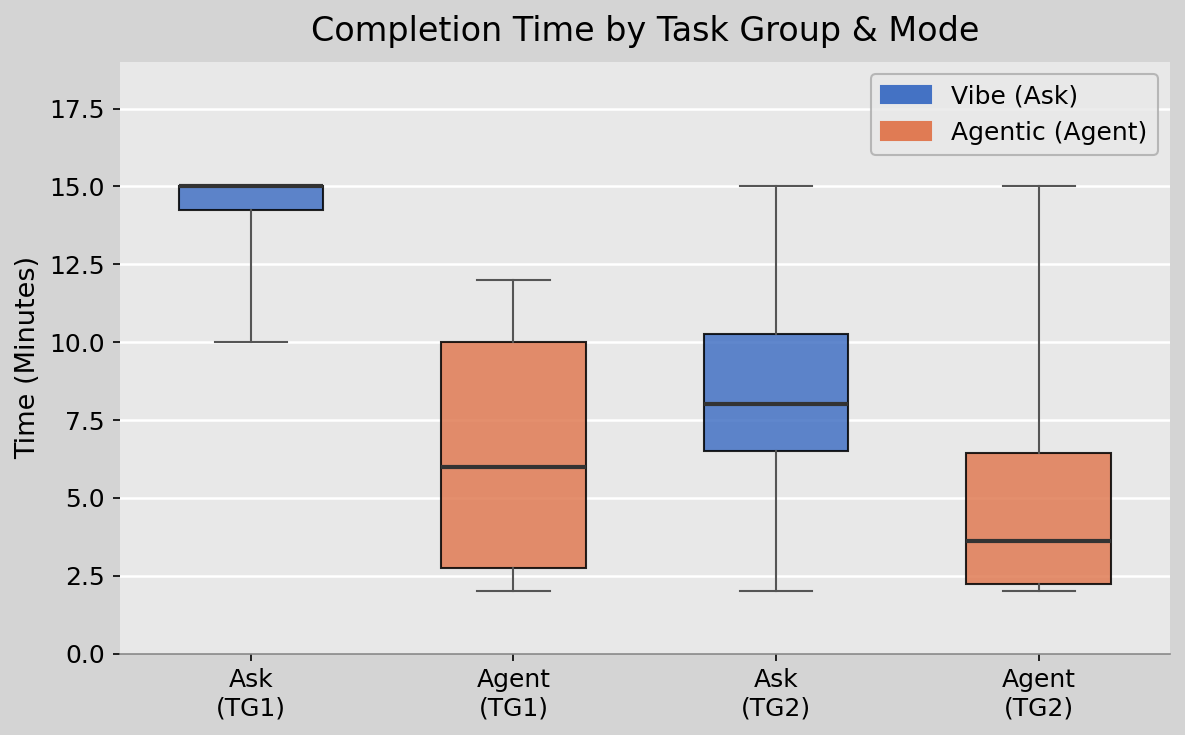
\includegraphics[width=0.8\textwidth]{figures/fig1_time.png}
  \caption[Completion Time by Task Group \& Paradigm]{Distribution of completion times by task group and coding paradigm. Agentic Coding shows consistently lower median times. In TG1, Vibe Coding times cluster near the 15-minute ceiling, reflecting frequent time-limit exhaustion; in TG2, both paradigms performed more similarly, though Agentic Coding retained a time advantage.}
  \label{fig:completion_time}
\end{figure}

\begin{table}[H]

  \centering

  \caption[RQ1 outcomes by task group]{RQ1 outcomes split by task group (TG1: data analysis; TG2: bug fixing). Completion time is in \textbf{minutes}. Each cell has $n=6$ observations.}

  \label{tab:rq1-by-taskgroup}

  \renewcommand{\arraystretch}{1.15}

  \rowcolors{2}{gray!10}{white}

  \begin{tabular*}{\textwidth}{@{\extracolsep{\fill}}llcc}

    \toprule

    \rowcolor{accentblue}

    \textbf{Task Group} & \textbf{Paradigm} & \textbf{Time (min; median [Q1, Q3])} & \textbf{Success (tasks; \%)} \\

    \midrule

    TG1 (Data analysis) & Vibe Coding & 15.0 [14.2, 15.0] & 2/6 (33\%) \\

    TG1 (Data analysis) & Agentic Coding & 6.0 [2.8, 10.0] & 4/6 (67\%) \\

    TG2 (Bug fixing) & Vibe Coding & 8.0 [6.5, 10.2] & 3/6 (50\%) \\

    TG2 (Bug fixing) & Agentic Coding & 3.6 [2.2, 6.5] & 5/6 (83\%) \\

    \bottomrule

  \end{tabular*}

\end{table}

\subsection{Task Success and Failure Cases}

Overall, Agentic Coding yielded a higher task success rate than Vibe Coding (Agentic: 9/12, 75\%; Vibe: 5/12, 42\%). Figure~\ref{fig:success_rates} shows the same pattern when stratified by task group: Agentic Coding achieved higher success in both TG1 (data analysis) and TG2 (bug fixing), with the gap being more pronounced in TG1.

\begin{figure}[H]
  \centering
  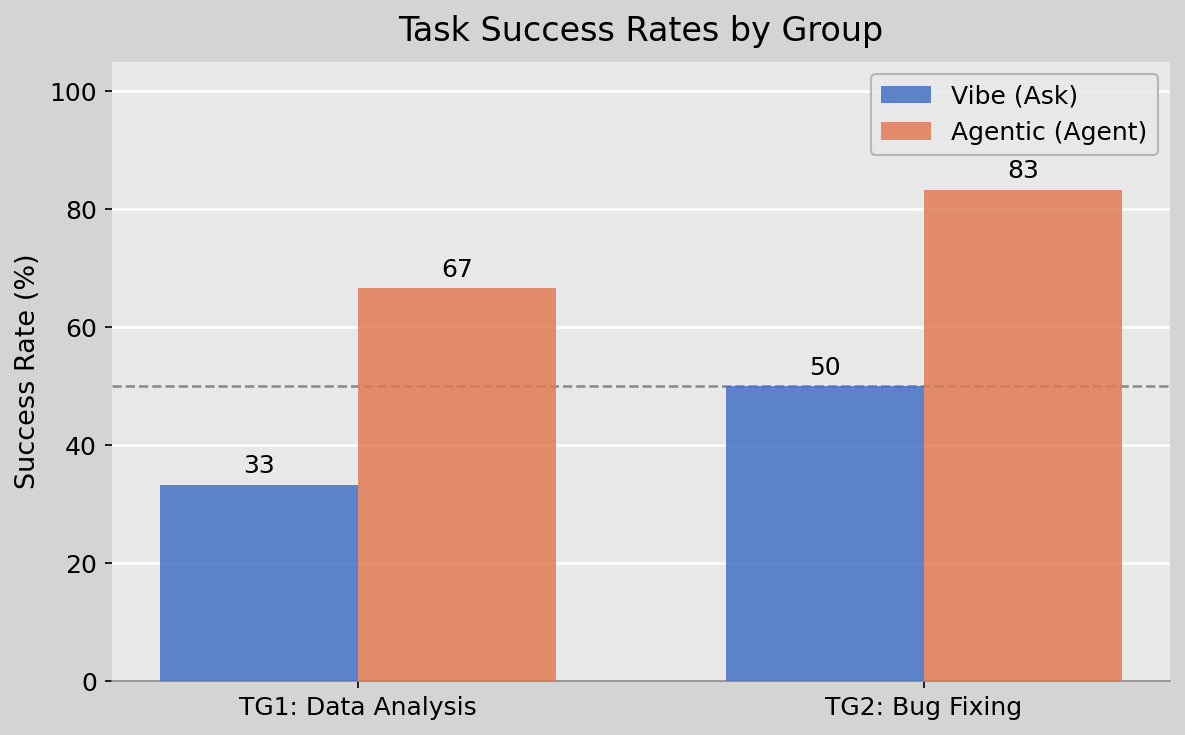
\includegraphics[width=0.7\textwidth]{figures/fig2_success.png}
  \caption[Task Success Rates]{Task success rates by task group. Bars show the percentage of tasks completed successfully within the time limit. Agentic Coding outperforms Vibe Coding in both task groups, with the advantage more pronounced in TG1. Each cell has $n=6$ observations.}
  \label{fig:success_rates}
\end{figure}

When viewed at the level of individual participants, six succeeded only under Agentic Coding, two succeeded only under Vibe Coding, three succeeded in both, and one failed in both. An exact McNemar test on the discordant pairs did not reach significance ($p=0.289$), consistent with the limited sample size.

Failure patterns differed by task group. In TG1, all four Vibe Coding failures coincided with the time ceiling, reflecting sustained prompt-and-repair cycles that prevented convergence on a correct implementation. Agentic Coding failures in TG1 were associated with environment or early-execution faults that consumed setup time. In TG2, Vibe Coding produced three failures, predominantly linked to accumulated implementation errors or environment issues that could not be resolved within the time limit. The single Agentic Coding failure in TG2 was similarly attributable to environment setup overhead rather than conceptual difficulty.

Partial progress was not quantified in the binary success metric, but session recordings captured intermediate states (e.g., reductions in failing tests) that informed the qualitative interpretation of failure cases.

\subsection{Interaction Cost: Prompts and Agent Runs}

Interaction cost captures the granularity of the work process: how many discrete interaction cycles were required to move from the initial task state to a solution (or to the time limit). Under Vibe Coding, each unit was a distinct prompt submitted by the participant; under Agentic Coding, each unit was an agent run (with review/approval decisions). Because one agent run can bundle multiple steps that would require several prompts in Vibe Coding, the comparison is interpreted as the number of discrete human--AI interaction cycles rather than a one-to-one mapping between prompts and runs.

As illustrated in Figure~\ref{fig:interaction_cost}, Agentic Coding required markedly fewer interaction units. The median was 1.5 runs (interquartile range [1, 3]) versus 5.0 prompts under Vibe Coding (Table~\ref{tab:rq1-overview}). A paired Wilcoxon signed-rank test confirmed that this reduction was statistically reliable ($V=0$, $p=0.0020$, rank-biserial $r=1.00$, showing a large effect).

\begin{figure}[H]
  \centering
  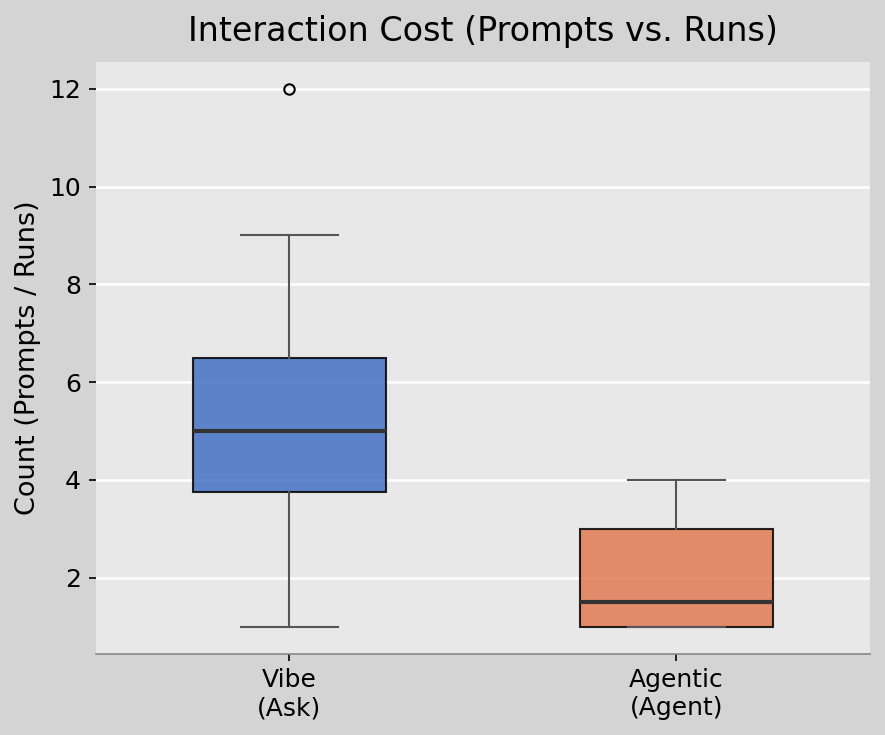
\includegraphics[width=0.6\textwidth]{figures/fig3_interaction.png}
  \caption[Interaction Cost Comparison]{Distribution of interaction costs by paradigm. Agentic Coding not only reduced the median cost but also compressed the variance in effort required.}
  \label{fig:interaction_cost}
\end{figure}

The difference was most pronounced in TG1, where Vibe Coding commonly triggered repeated prompt-and-repair cycles that each added an interaction unit and rarely converged within the time limit. Agentic Coding more often converged in a small number of multi-step runs. In TG2, Agentic Coding continued to require fewer interaction cycles, and its higher success rate (83\% vs.\ 50\%) suggests that lower interaction cost translated into more reliable task completion.

Interaction cost was positively associated with completion time across all observations (Spearman's $\rho=0.68$, $p<0.001$). This association is descriptive rather than causal; both metrics likely co-vary with task difficulty and recovery effort.

\subsection{Interruptions and Flow Breaks}

The final quantitative measure addressing RQ1 focused on interruptions, coded using the operational definition described in Section~\ref{sec:measures}. In short, interruptions capture moments where visible progress stalls due to uncertainty, tool friction, or recovery work.

Across all participants, Vibe Coding exhibited more interruptions than Agentic Coding. The median interruption count under Vibe Coding was 1 (interquartile range [0, 1]), compared to 0 under Agentic Coding (interquartile range [0, 0]; Table~\ref{tab:rq1-overview}). A Wilcoxon signed-rank test confirmed this reduction ($V=0$, $p=0.016$, rank-biserial $r=1.00$, denoting a large effect among non-tied pairs).

The qualitative character of interruptions differed by paradigm. Under Vibe Coding, interruptions typically coincided with the prompt-and-repair cycle: the pause between receiving an inadequate response and formulating the next prompt represented a break in forward progress. Under Agentic Coding, interruptions more often reflected supervision friction (monitoring an agent run, noticing drift, reviewing a larger diff before approval, or stepping in to course-correct).

Interruptions were most visible in TG1, where the more exploratory task structure created more opportunities for misalignment and recovery. In TG2, interruptions were less common overall, though the general pattern held.

% ---------------------------------------------------------

\section{Qualitative Results (RQ2: Trust, Control, and Workflow Fit)}

While the quantitative results capture efficiency and disruption outcomes, they do not fully represent how participants experienced working with the two paradigms. Research Question~2 explored how participants perceived and navigated trust, control, and workflow fit. This section combines post-session interviews and field notes.

\subsection{Coding Approach for Qualitative Data}

The qualitative analysis drew on post-session semi-structured interviews and structured observational notes anchored to specific moments in the recordings. Coding followed a deductive--inductive process: initial categories mapped to the study constructs (trust, control, workflow fit, flow), then expanded with subcodes that emerged from the data (e.g., delegation comfort, approval friction, confidence shifts). Episodes were selected based on their clarity, specificity to a concrete task moment, and recurrence across participants.

\subsection{Perceived Control and Oversight}

A consistent theme concerned the nature of control. Rather than treating control as present in one paradigm and absent in the other, participants described different control \emph{mechanisms} and different points of intervention.

Descriptively, 7 out of 12 participants leaned toward Agentic Coding as enabling better overall control, but qualified this by explaining that the control was different in nature. Agentic Coding reduced micro-decisions and shifted effort into oversight (monitoring runs, reviewing diffs, approving/rejecting actions, and intervening when the agent drifted). Several participants described this supervisory stance as efficient and empowering; others found it cognitively taxing, especially when they were unsure about what the agent was doing or why.

Vibe Coding was consistently described as supporting step-by-step steering. Participants appreciated being able to request smaller changes, inspect outputs incrementally, and correct direction early. However, when many iterations were required, the mental effort of deciding what to ask next and integrating fragmented outputs became burdensome, often embodying the prompt-and-repair cycle described in Section~\ref{sec:rq1}.

Overall, control was experienced as distributed distinctly across the task: steering in Vibe Coding versus supervision in Agentic Coding. Preferences depended on working style, confidence in reviewing larger diffs, and perceived task ambiguity.

\subsection{Trust Calibration and Verification Behavior}

Trust emerged as active and behaviorally grounded in verification strategies rather than as blanket acceptance. Across the two paradigms, participants rarely relied on the AI uncritically. Instead, they calibrated trust based on observed performance, clarity of reasoning, and, most prominently, test feedback.

Descriptively, 8 out of 12 participants reported higher confidence in Agentic Coding outcomes, often attributing this to coherent, multi-step attempts that reduced fragmentation. When an agent run produced a passing solution, participants interpreted it as evidence that the agent captured the task end-to-end.

At the same time, participants emphasized that Agentic Coding needed careful verification precisely because the AI had more autonomy. Larger multi-step changes increased the perceived risk of unintended consequences, and several participants described heightened diligence when reviewing diffs before approval (``approval anxiety''). Under Vibe Coding, confidence was frequently tied to incremental transparency: smaller changes felt easier to judge locally, even when progress was slower.

Across both models, \texttt{pytest} served as the primary verification anchor. Passing tests increased confidence; failing tests triggered strategy modifications (tightening requirements, reducing scope, or re-checking assumptions). Participants explicitly described confidence shifting after early errors or drift, leading to tighter oversight behaviors (more frequent tests, smaller requested steps, or greater constraints on what the AI should change).

\subsection{Workflow Fit and Perceived Flow}

Workflow fit captures whether a coding paradigm felt compatible with how participants prefer to work, while flow captures whether the interaction sustained focus and continued progression. These two perceptions are related but not identical: a paradigm can feel efficient yet still feel mentally disruptive.

\paragraph{Descriptive ratings.}
Figure~\ref{fig:likert_ratings} and Table~\ref{tab:rq2-likert} summarize post-task ratings (1--5). The clearest separation is on perceived efficiency: Agentic Coding scored higher ($M=4.75$, $SD=0.62$) than Vibe Coding ($M=4.00$, $SD=1.48$), and with notably less variance, meaning participants agreed more consistently that it felt efficient. Flow and focus tell a different story: the two paradigms scored almost identically (Vibe: $M=3.17$; Agentic: $M=3.08$), meaning that being faster did not translate into feeling more in the zone. Workflow fit was similarly close (Vibe: $M=3.67$; Agentic: $M=3.42$), but Agentic Coding showed much higher variability ($SD=1.62$ vs.\ $1.15$), reflecting that some participants found it a natural fit while others did not.

\begin{figure}[H]
  \centering
  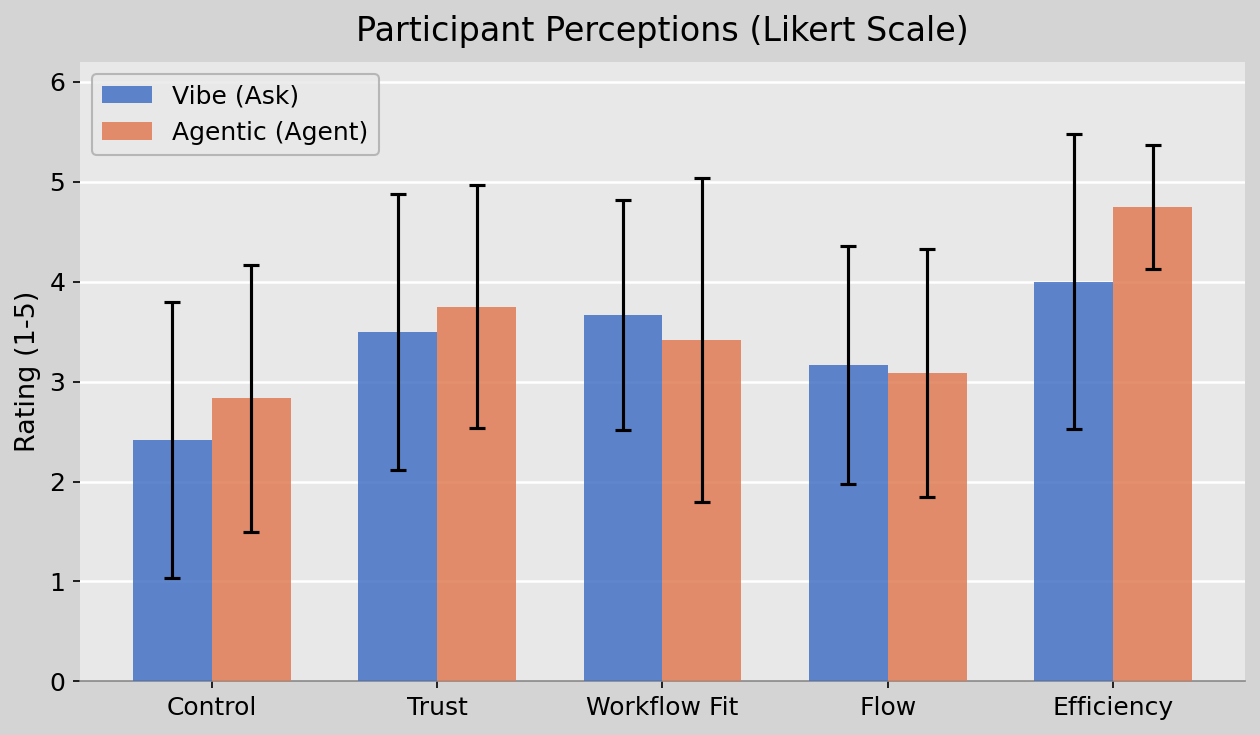
\includegraphics[width=0.9\textwidth]{figures/fig4_likert.png}
  \caption[Post-Task Likert Ratings]{Participant perceptions of the two coding paradigms (1--5). Error bars represent standard deviations. The largest separation appears for perceived efficiency; flow/focus and workflow fit show overlapping means with substantial variance.}
  \label{fig:likert_ratings}
\end{figure}

\begin{table}[H]
  \centering
  \caption[Post-task Likert ratings by paradigm]{Post-task Likert ratings (1--5) by paradigm across all task observations ($n=12$ per paradigm). Items correspond to perceived control/oversight, trust/confidence, workflow fit, flow/focus, and perceived efficiency.}
  \label{tab:rq2-likert}
  \renewcommand{\arraystretch}{1.15}
  \rowcolors{2}{gray!10}{white}
  \begin{tabular}{lcc}
    \toprule
    \rowcolor{accentblue}
    \textbf{Item (1--5)} & \textbf{Vibe Coding (mean, SD)} & \textbf{Agentic Coding (mean, SD)} \\
    \midrule
    Control / oversight & 2.42 (1.38) & 2.83 (1.34) \\
    Trust / confidence & 3.50 (1.38) & 3.75 (1.22) \\
    Workflow fit & 3.67 (1.15) & 3.42 (1.62) \\
    Flow / focus & 3.17 (1.19) & 3.08 (1.24) \\
    Perceived efficiency & 4.00 (1.48) & 4.75 (0.62) \\
    \bottomrule
  \end{tabular}
\end{table}

\paragraph{Interview synthesis.}

Interview responses help explain why efficiency was separated while flow and fit were not. In interviews, 10 out of 12 participants described Agentic Coding as more efficient overall, consistent with the quantitative reductions in completion time and interaction cost reported for RQ1. However, several participants noted that efficiency gains came with a different ``feel'' of working: instead of continuous hands-on progress, Agentic Coding sometimes shifted attention into supervision (waiting for runs, reviewing larger diffs, and intervening when drift occurred). By contrast, Vibe Coding was often described as more stepwise and transparent, supporting continuous engagement, but at the cost of conversational overhead (repeated prompt formulation and context re-establishment).

Participants also reported that workflow fit could vary by task. Agentic Coding was generally preferred for well-defined tasks where delegation felt safe, whereas Vibe Coding was sometimes preferred for more ambiguous or higher-stakes moments where tight steering felt more comfortable. These comments correspond to the higher variability in workflow-fit ratings under Agentic Coding ($SD=1.62$ vs.\ $1.15$), suggesting the paradigm fit some participants strongly while feeling mismatched for others.

\paragraph{Methodological note on Likert analysis.}

Given the ordinal nature of Likert-scale data and the small sample ($n=12$), these ratings are treated as descriptive summaries rather than as the basis for formal inferential testing. Differences between paradigms on control, trust, workflow fit, and flow are small relative to within-group variability. Perceived efficiency is the clearest separation both in mean and variance (Table~\ref{tab:rq2-likert}), which is consistent with the quantitative efficiency results reported for RQ1.

The next chapter interprets these outcomes in relation to prior literature and develops their consequences for the collaboration--delegation trade-off in AI-assisted coding. These interpretations form the foundation for the best practices proposed in Chapter~\ref{chap:conclusion}.
